\documentclass[11pt,a4paper]{article}

\usepackage[utf8]{inputenc}
\usepackage[T1]{fontenc}
\usepackage{lmodern}
\usepackage[french]{babel}
\usepackage[margin=2.1cm]{geometry}
\usepackage{microtype}
\usepackage{booktabs}
\usepackage{array}
\usepackage[table]{xcolor}
\usepackage{graphicx}
\usepackage{caption}
\usepackage[most]{tcolorbox}

\definecolor{navy}{HTML}{1F3864}
\definecolor{bluemid}{HTML}{2E5496}
\definecolor{lightblue}{HTML}{D6E0F0}

\captionsetup{font=small,labelfont={bf,color=navy},labelsep=period}
\graphicspath{{../figures/}}

\newtcolorbox{cle}[1][]{colback=lightblue!40,colframe=navy,boxrule=0.6pt,
  arc=2pt,left=8pt,right=8pt,top=6pt,bottom=6pt,#1}

\title{\vspace{-1.2cm}\color{navy}\bfseries Piliers en bout de chaîne\\[2pt]
  \large Vue complémentaire à la carte de criticité}
\author{Kélian Kaddouri}
\date{20 juillet 2026}

\begin{document}
\maketitle
\vspace{-0.9cm}

\begin{cle}
\textbf{Ce que la carte de criticité ne dit pas.} Elle répond à deux questions :
quel pilier \textbf{amorce} une cascade, et quelle \textbf{gravité} elle atteint. Elle
ne dit pas où la cascade \textbf{s'arrête}. Ce tableau complète la vue : pour chaque
pilier, sa propension à être en \textbf{bout de chaîne} (aller \og{}vers rien\fg{})
plutôt qu'à propager. Un pilier qui pousse peu vers les autres (faible force sortante)
est le plus souvent terminal.
\end{cle}

\medskip
\begin{center}
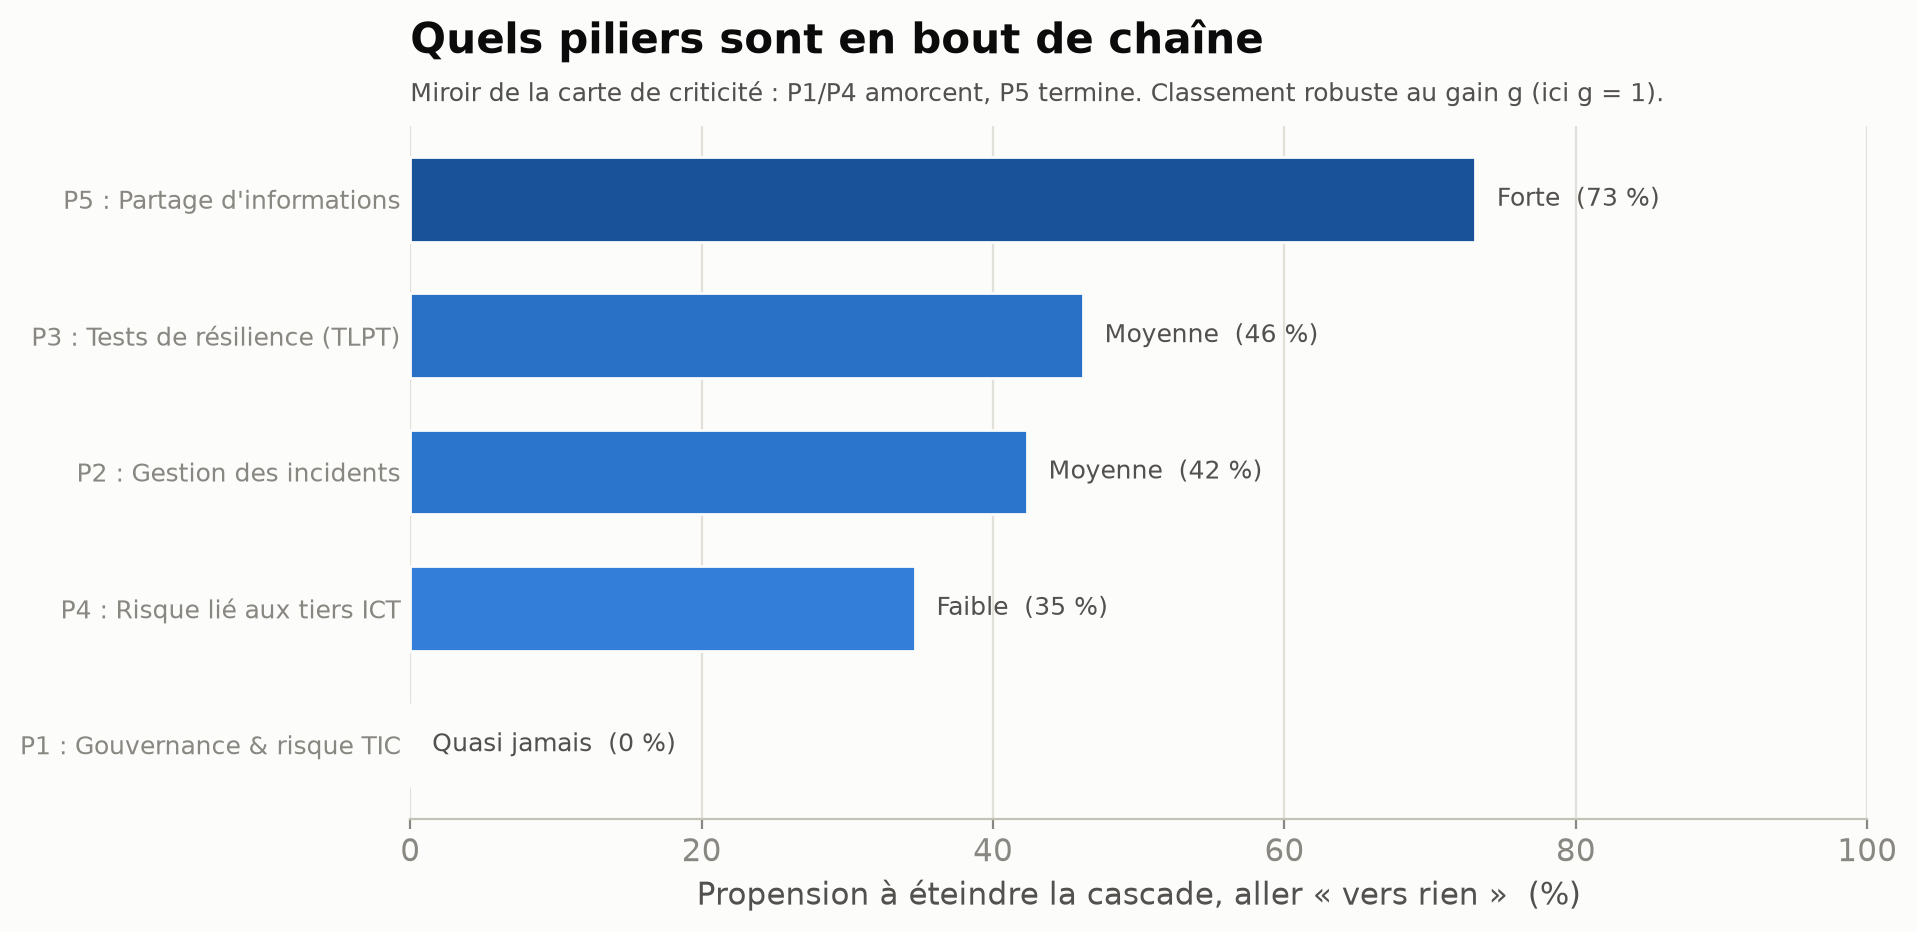
\includegraphics[width=0.86\linewidth]{F13_bout_de_chaine.png}
\captionof{figure}{Propension de chaque pilier à terminer la cascade. \textbf{P5} (partage
d'informations) est le terminal typique : il éteint la cascade environ trois fois sur
quatre. \textbf{P1} (gouvernance) ne termine quasi jamais, il reste en amont. C'est
l'image miroir de la carte de criticité, où P1 et P4 dominent comme amorces.}
\end{center}

\begin{center}
\small
\renewcommand{\arraystretch}{1.16}
\begin{tabular}{@{}l c c l@{}}
\toprule
\textbf{Pilier} & \textbf{Force sortante $s_j$} & \textbf{Propension à terminer} & \textbf{Niveau} \\
 & \footnotesize somme des liens sortants & \footnotesize cas de référence $g=1$ & \\
\midrule
P5 : Partage d'informations      & $0{,}70$ & $73\,\%$ & \textbf{Forte} \\
P3 : Tests de résilience (TLPT)   & $1{,}40$ & $46\,\%$ & Moyenne \\
P2 : Gestion des incidents        & $1{,}50$ & $42\,\%$ & Moyenne \\
P4 : Risque lié aux tiers ICT     & $1{,}70$ & $35\,\%$ & Faible \\
P1 : Gouvernance \& risque TIC    & $2{,}60$ & $0\,\%$  & Quasi jamais \\
\bottomrule
\end{tabular}
\captionof{table}{Du plus terminal au moins terminal. La force sortante et la propension à
terminer varient en sens inverse.}
\end{center}

\begin{cle}
\textbf{Ce qui est défendable : le classement, pas le pourcentage.} La propension à
terminer s'écrit $\text{term}_j = 1 - g\,\dfrac{s_j}{\max_k s_k}$. Le gain de contagion
$g$ multiplie toutes les propensions à propager : il déplace les niveaux sans jamais
changer leur ordre. Le classement $\text{P5} > \text{P3} > \text{P2} > \text{P4} >
\text{P1}$ est donc \textbf{invariant} au seul paramètre non calibré du bloc de
propagation. Les valeurs en \% valent au cas de référence $g=1$, cohérent avec l'état
d'arrêt présenté dans les slides.
\end{cle}

\smallskip
\noindent\footnotesize\textcolor{navy}{\textbf{Méthode.}} $s_j$ est la somme des forces
sortantes $\text{TRANS}[j][\cdot]$ (jugement d'expert, source unique
\texttt{cascade\_model} ; figure \texttt{build\_bout\_de\_chaine.py}). Sortie
\textbf{qualitative} : une vraisemblance d'être terminal, pas une probabilité estimée sur
données.

\end{document}
